\documentclass[border=3pt]{standalone}

%%Fonts
%\usepackage{fontspec}
%\setmainfont[Mapping=tex-text]{JetBrains Mono}

% Tikz
\usepackage{tikz}
\usetikzlibrary{calc, positioning}

\tikzset{
node distance = 1.5cm and 1.5cm,
state/.style={
	draw,
	very thick,
	shape=circle, 
	inner sep=0pt,
	outer sep=2pt,
	text width=25pt,
	align=center,
	fill=gray!30,
},
S0/.style={
	draw=gray!100,
	fill=gray!20,
},
S1/.style={
	draw=green!70!black,
	fill=green!20,
},
S2/.style={
	draw=magenta!100,
	fill=magenta!20,
},
S3/.style={
	draw=cyan!100,
	fill=cyan!20,
},
S4/.style={
	draw=orange!100,
	fill=orange!20,
},
connection/.style={
	-stealth,
},
label/.style={
	font=\tiny\ttfamily,
	align=center,
}
}

% Notation
\usepackage{amsmath}

\begin{document}
	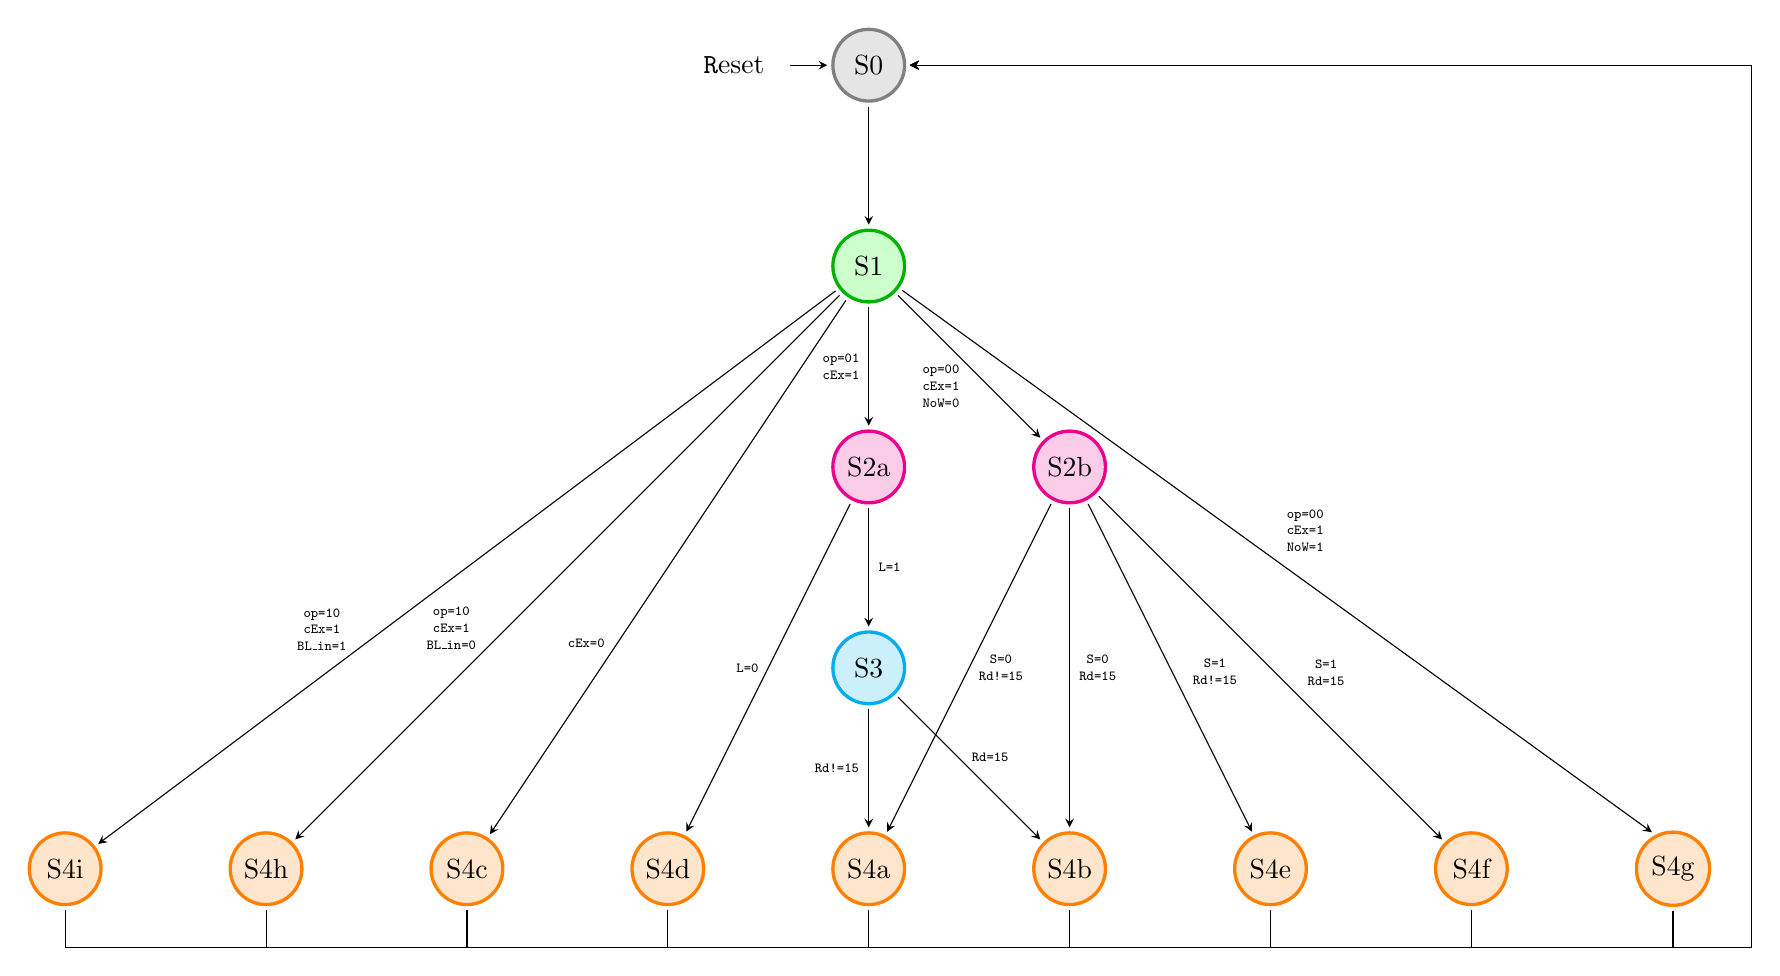
\begin{tikzpicture}
		% State 0
		\node[state, S0] (S0) {S0};
		% State 1
		\node[state, below = of S0, S1] (S1) {S1};
		% State 2
		\node[state, below = of S1, S2] (S2a) {S2a};
		\node[state, right = of S2a, S2] (S2b) {S2b};
		% State 3
		\node[state, below = of S2a, S3] (S3) {S3};
		% State 4
		\node[state, below = of S3, S4] (S4a) {S4a};
		%% Right
		\node[state, right = of S4a, S4] (S4b) {S4b};
		\node[state, right = of S4b, S4] (S4e) {S4e};
		\node[state, right = of S4e, S4] (S4f) {S4f};
		\node[state, right = of S4f, S4] (S4g) {S4g};
		%% Left
		\node[state, left = of S4a, S4] (S4d) {S4d};
		\node[state, left = of S4d, S4] (S4c) {S4c};
		\node[state, left = of S4c, S4] (S4h) {S4h};
		\node[state, left = of S4h, S4] (S4i) {S4i};
		
		% Connections
		
		% Reset
		\draw[connection] (-1,0) -- (S0) node[pos=-1.5] {\texttt Reset};
		
		% S0 ->
		\draw[connection] (S0) -- (S1);
		
		% S1 ->
		\draw[connection] (S1) -- (S2a) 
			 node[label, pos = 0.5, xshift=-10] {op=01\\cEx=1};
		\draw[connection] (S1) -- (S2b)
			 node[label, pos = 0.5, anchor=35] {op=00\\cEx=1\\NoW=0};
		\draw[connection] (S1) -- (S4g.120) 
			 node[label, pos = 0.5, anchor=south west] {op=00\\cEx=1\\NoW=1};
			 
		\draw[connection] (S1) -- (S4c) 
			 node[label, pos = 0.65, anchor=base east] {cEx=0};
		\draw[connection] (S1) -- (S4h) 
			 node[label, pos = 0.65, anchor=base east] {op=10\\cEx=1\\BL\_in=0};
		\draw[connection] (S1) -- (S4i)
			 node[label, pos = 0.65, anchor=base east] {op=10\\cEx=1\\BL\_in=1};
			 
		% S2a ->
		\draw[connection] (S2a) -- (S3)
			 node[label, pos = 0.5, right] {L=1};
		\draw[connection] (S2a) -- (S4d)
			 node[label, pos = 0.5, left] {L=0};
		
		% S2b ->
		\draw[connection] (S2b) -- (S4a)
			 node[label, pos = 0.5, right] {S=0\\Rd!=15};
		\draw[connection] (S2b) -- (S4b)
			 node[label, pos = 0.5, right] {S=0\\Rd=15};
		\draw[connection] (S2b) -- (S4e)
			 node[label, pos = 0.58, above right] {S=1\\Rd!=15};
		\draw[connection] (S2b) -- (S4f)
			 node[label, pos = 0.58, above right] {S=1\\Rd=15};
			 
		% S3 -> 
		\draw[connection] (S3) -- (S4a)
			 node[label, pos = 0.5, left] {Rd!=15};
		\draw[connection] (S3) -- (S4b)
			 node[label, pos = 0.45, anchor=base west] {Rd=15};
		
		
		% S4g ->
		\draw[connection] (S4g) -- ++(0,-1) -| ++(1,0) coordinate (S4g_temp) -- 
						  (S0-|S4g_temp) coordinate (S4g_temp) -- (S0);
		
		% S4f ->
		\draw[connection] (S4f) -- ++(0,-1) -| (S4g_temp) -- (S0);		
		
		% S4e ->
		\draw[connection] (S4e) -- ++(0,-1) -| (S4g_temp) -- (S0);		
		
		% S4b ->
		\draw[connection] (S4b) -- ++(0,-1) -| (S4g_temp) -- (S0);
		
		% S4a ->		
		\draw[connection] (S4a) -- ++(0,-1) -| (S4g_temp) -- (S0);
		
		% S4d ->
		\draw[connection] (S4d) -- ++(0,-1) -| (S4g_temp) -- (S0);
		
		% S4c ->
		\draw[connection] (S4c) -- ++(0,-1) -| (S4g_temp) -- (S0);
		
		% S4h ->
		\draw[connection] (S4h) -- ++(0,-1) -| (S4g_temp) -- (S0);
		
		% S4i ->
		\draw[connection] (S4i) -- ++(0,-1) -| (S4g_temp) -- (S0);
	\end{tikzpicture}
\end{document}